%pic2,pic3
%
Es wurde versucht mittels verschiedenen Versuchsanordungen Leerlaufspannung und Innenwiderstand
verschiedener Spannungsquellen zu bestimmen. Zu beginn wurde die Leerlaufspannung einer Monozelle
direkt mit einem Spannungsmessgerät gemessen. Danach wurden komplexere Versuchsmethoden durchgeführt.
\subsection{Monozelle mit Verbraucher}
	\begin{figure}[h]
		\begin{center}
		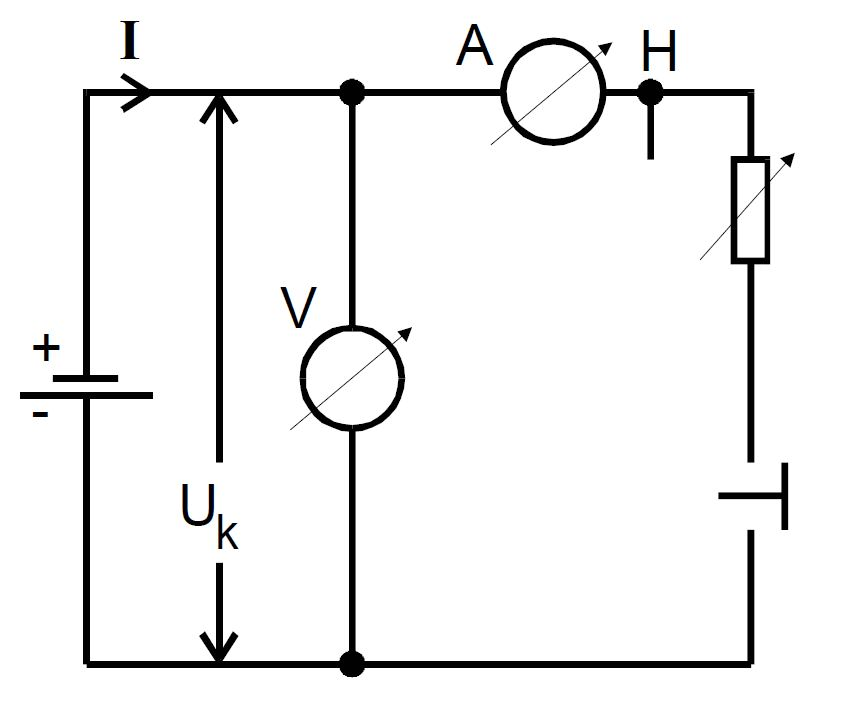
\includegraphics[scale=0.3]{pic2.jpg}
		\caption{Versuchsanordnung 1 [1]}
		\label{pic2}
		\end{center}	
	\end{figure}
Es wurde ein Schaltkreis wie in Abbildung \ref{pic2} aufgebaut. Dann ist bei Variation des 
Belastungswiderstandes jeweils die Spannung $U_k$ und der Stromfluss $I$ abgelesen worden.
\FloatBarrier
\subsection{Monozelle mit Verbraucher und Gegenspannung}
	\begin{figure}[h]
		\begin{center}
		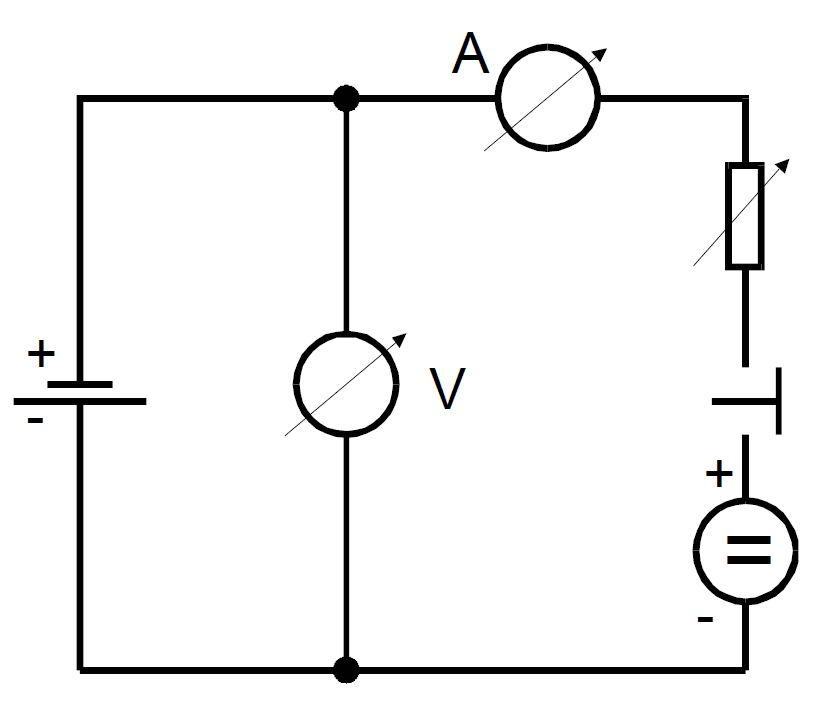
\includegraphics[scale=0.3]{pic3.jpg}
		\caption{Versuchanordnung 2 (mit Gegenspannung) [1]}
		\label{pic3}
		\end{center}	
	\end{figure}
Nun wurde der Schaltkreis mit einer Gegenspannung erweitert (Abb. \ref{pic3}).
Anschließend wurde bei konstanter Gegenspannung abermals $U_k$ in Abhängigkeit von $I$ abgelesen.
\FloatBarrier
\subsection{Sinus- und Rechteckspannung mit Verbraucher}
Abermals wurde ein Schaltkreis wie in Abbildung \ref{pic2} aufgebaut, diesmal wurde statt der 
Monozelle ein RC-Generator als Spannungsquelle eingebaut. Dann wurde in passendem Frequenzbereich 
jeweils bei Rechteck- und Sinusspannung abermals $U_k$ abhängig von $I$ unter Variation des
Belastungswiderstandes gemessen.